\subsection{Greedy Best First Search (GBFS) Algorithm }
\subsubsection*{Concepts}
\begin{itemize}
    \item \textbf{Introduction:} Greedy Best First Search (GBFS) is a graph search algorithm that expands the most promising node chosen according to a heuristic function. It does not guarantee optimal solutions but is often efficient in practice for certain types of problems.
    \item \textbf{Traversal Method:} GBFS uses a priority queue ordered by the heuristic value to expand nodes with the most promising estimated cost.
\end{itemize}
\subsubsection{Heuristic function note}

Due to the requirements of this project, the lecturer specified that the heuristic function should be the edge weight, which initially caused some confusion for me.

\begin{figure}[h]
\centering
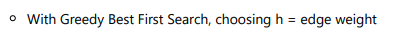
\includegraphics[]{Greedy_requirement.PNG}
\label{fig:Greedy_requirement}
\end{figure}

Therefore, I have decided to use the edge weight as the heuristic function, representing the direct distance between the current node and the goal node.

The heuristic function is defined as follows:
\[h[node] = matrix[goal][node]\]


\subsubsection*{Pseudo Code}
function BEST-FIRST-SEARCH(problem, f) was mentioned in Section \ref{UCS_best_first_search}.
\begin{verbatim}
function GREEDY-BEST-FIRST-SEARCH(problem) returns a solution node or failure
    return BEST-FIRST-SEARCH(problem, HEURISTIC)

\end{verbatim}

\subsubsection*{Complexity}
\begin{itemize}
    \item \textbf{Time Complexity:} The worst-case time complexity of GBFS is \( O(|V|) \), where \( V \) is the number of vertices. With a good heuristic function, however, the complexity can be substantially reduced, potentially reaching \( O(b^m) \) on certain problems, where \( b \) is the branching factor and \( m \) is the maximum depth of the search.
    \item \textbf{Space Complexity:} GBFS has a space complexity of \( O(|V|) \), primarily due to the priority queue and the visited set.
\end{itemize}

\subsubsection*{Properties}
\begin{itemize}
    \item \textbf{Completeness:} GBFS is complete in finite state spaces but may not be complete in infinite state spaces due to the potential for encountering loops or cycles.
    \item \textbf{Optimality:} GBFS is not generally optimal because it does not consider the total path cost but relies solely on the heuristic function to guide the search.
    \item \textbf{Traversal Type:} GBFS explores nodes based on the heuristic value, prioritizing nodes that appear to be closest to the goal according to the heuristic.
\end{itemize}